\chapter{Project documents}
\label{appendix-project-documents}
Documents produced in relation to the project will be presented in this section. Both status reports and activity plans were to be created and delivered to the supervisor every other week. 

\section{Status report example}
Below is a copy of a status report made by the group for the supervisor. This status report encompasses both week 6 and 7.\\
\newline

\textbf{1. Introduction}\\
These two weeks were the first weeks of project work, since little could be done prior to meeting the customer. During the first week there was one member missing.\\
\newline

\textbf{2. Progress summary}\\
In this two-week period we have completed on average 68\% of the work scheduled on the activity plan. We believe that we still are on schedule. The work that was done was in general related to the design of the final product and making sure we have all the required libraries, licenses and other factors that need to be in order before we start programming the actual product.\\
\newline

\textbf{3. Open / closed problems}\\
\newline
\textbf{Open:}
\begin{itemize}
	\item{New requirement: friendlier bluetooth device pairing}
	\item{Bluetooth connection: need to add a bluetooth module to the arduino}
	\item{Non-documented preexisting code}
	\item{Product naming}
\end{itemize}
\vspace{8mm}

\textbf{Closed:}
\begin{itemize}
	\item{Lacking source code: Will not use the compiled program in question}
	\item{Licenses: separate out licensed components into separate projects}
\end{itemize}
\vspace{8mm}

\textbf{4. Planned work for the next period}\\
For the next period we will have to complete the designs of the project and complete version 0.1 to show to the customer.\\
\newline

\textbf{5. Updated risks analysis}\\
\begin{itemize}
	\item{License incompatibility: impact has gone down from 8 to 7. Importance has gone down from 10 to 8. This is because of information from the customer regarding ways to circumvent this issue (as mentioned above).}
\end{itemize}

\section{Activity plan example}
Below is an example of an activity plan made by the group for the supervisor. This activity plan spans weeks 6 and 7.\\

\begin{figure}[H]
\makebox[\textwidth][c]{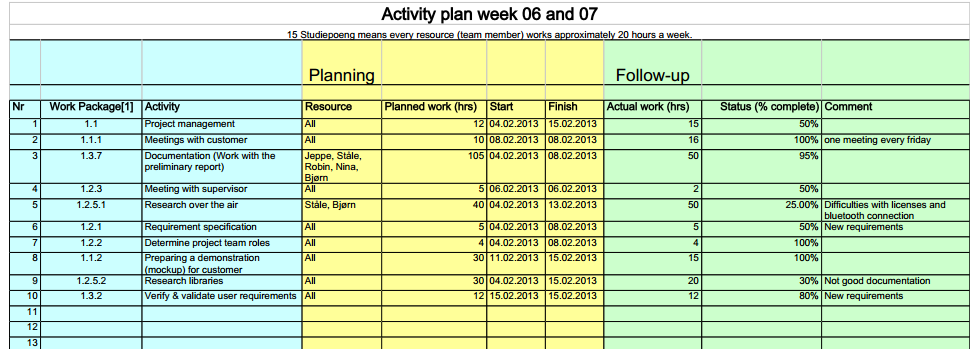
\includegraphics[width=1.3\textwidth]{images/activity_plan_example.png}}
\caption{Example of activity plan for the weeks 6 and 7}
\end{figure}
